\documentclass[12pt]{article}
\usepackage[utf8]{inputenc}
\usepackage[T1]{fontenc}
\usepackage{titlesec}
\usepackage{listings}
\usepackage{graphicx}
\usepackage{float}
%\usepackage{babel}[it]
% Redefine \ttvar to enable wrapping

\newcommand*\ttvar[1]{\texttt{\expandafter\dottvar\detokenize{#1}\relax}}
\newcommand*\dottvar[1]{\ifx\relax#1\else
  \expandafter\ifx\string.#1\string.\allowbreak\else#1\fi
  \expandafter\dottvar\fi}
\renewcommand{\theparagraph}{\Alph{paragraph}}

\titleformat{\subsubsection}[runin]{\normalfont\bfseries}{\thesubsubsection}{1em}{}[]
\renewcommand{\thesubsubsection}{\arabic{section}.\ifnum\value{subsection}>0{\arabic{subsection}.}\fi\Alph{subsubsection}}

\setcounter{tocdepth}{3}

\title{Peer-Review 2: Network}
\author{Berardinelli, Genovese, Grandi, Haddou\\Gruppo AM21}

\begin{document}

\maketitle
\begin{center}
Peer review del protocollo di rete del gruppo AMXX 
\end{center}

\tableofcontents
\newpage
% -------------
% LATI POSITIVI
% -------------

\section{Lati positivi}
\subsection{Chiarezza del diagramma presentato}
Il diagramma presentato è tutto sommato abbastanza chiaro e gestisce la quasi totalità delle meccaniche di gioco. 

\section{Scelta del gameId}
% -------------
% LATI NEGATIVI
% -------------

\addtocontents{toc}{\setcounter{tocdepth}{2}}
\section{Lati negativi}
Raccogliamo qui una serie di appunti, nella speranza che risultino d'aiuto al gruppo in sede di valutazione del progetto.  

\subsection{Note sulla rappresentazione del diagramma}
 \subsubsection{Sequence diagram connessione TCP}
 Il sequence diagram UML per la connessione TCP presenta talvolta delle invocazioni di metodi fra gli attori \ttvar{Client} e \ttvar{Server}. La rappresentazione è errata poichè TCP non permette la \textit{remote method invocation}. Sarebbe opportuno mostrare il messaggio che viene inviato da client a server tramite \textit{socket}, modellando il \textit{controller} come un altro attore per evidenziarne -- fra il server e questo -- l'invocazione dei metodi, le return effettuate o le eccezioni tirate al server e gli specifici messaggi che vengono inviati da quest'ultimo al client nei vari casi.
 \subsubsection{Sequence diagram connessione RMI}
 Dualmente a come scritto in \textbf{2.1.A}, il sequence diagram UML per la connessione RMI presenta talvolta dei messaggi. Poichè il protocollo RMI non contempla listener di messaggi, al posto di messaggi di conferma o errore, dovrebbero essere riportate le return dei metodi o le eccezioni tirate dai metodi del controller.

\subsubsection{Loop, flow alternativi e opzionali} 
\begin{enumerate}
    \item Non sono indicate nel diagramma quali parti della sequenza si ripetano e fino a quali condizioni.
    \item Talvolta sono indicate sullo stesso messaggio situazioni alternative e mutualmente esclusive che probabilmente sono gestite da ognuno degli attori in modo differente.  
    \item Se fosse meglio dettagliata, alcune parti della sequenza di messaggi/invocazioni di metodi sarebbero da intendersi come opzionali.
\end{enumerate}

Lo standard del sequence diagram UML mette a disposizione blocchi grafici per situazioni iterative, alternative mutualmente esclusive e condizionali. Si potrebbero inserire nel diagramma per documentare in modo più preciso le singole situazioni.

\subsubsection{Distinzione fra messaggi sincroni e asincroni}
I messaggi e le chiamate sincrone o asincrone utilizzano nei diagrammi lo stesso puntatore. Lo standard UML ne prevede due diversi per i due tipi di messaggio/chiamata.

 \subsubsection{Situazioni non modellate}
 \begin{itemize}
     \item Il messaggio di \ttvar{placeCard} non contempla un messaggio di errore.
     Abbiamo ipotizzato la validazione potesse avvenire lato client ma ci è sembrato uno scenario poco auspicabile, in cui sarebbe facile modificare un client in modo tale da invalidare lo stato di gioco nel server.
     \item Non è contemplata una fase di scelta della faccia della starter card da piazzare sul tabellone di gioco. Abbiamo ipotizzato potesse avvenire con una \ttvar{placeCard} ma non ci sarebbe nessun modo, che sia descritto, per garantire lato server che questa sia piazzata per prima. 
     \item Non sono modellate le situazioni in cui il client deve scegliere degli oggetti fra un pool di possibili, come ad esempio le carte obiettivo. Come viene comunicato al client quali fra le due deve scegliere? Inoltre dopo la \ttvar{drawCard()} non sembra venga comunicato al client che carta viene pescata, in quanto viene inviato solo una conferma/errore. \textit{•}
 \end{itemize}
 
 \subsubsection{Nits}
 \begin{itemize}         
     \item La presenza dello \ttvar{stub} all'interno del diagramma dedicato alla versione RMI del protocollo ci sembra ridondante. Vengono utilizzati gli stessi messaggi (vedere \textbf{2.1.B}) sia a sinistra che a destra di questo.
     \item Dato che la scelta di una \ttvar{SecretObjectiveCard} avviene fra un paio di carte, sarebbe meglio modellizzarla con un \textit{boolean} chiamato ad esempio \ttvar{first} .
 \end{itemize}
 
\subsection{Livello di dettaglio del diagramma} Talvolta il diagramma non è particolarmente meticoloso nel dettagliare le interazioni fra gli attori coinvolti. Sottolineamo che lo scopo della documentazione è quello di redigere minuziosamente il protocollo prima di implementarlo, pensando a tutti gli edge case del caso e come vengono gestiti in modo isolato l'uno dall'altro. 

\subsubsection{Conferme e discriminazione degli errori} Se come gruppo pensiamo che per le conferme non siano necessarie particolari descrizioni, crediamo che gli errori potrebbero essere meglio differenziati per garantire una esperienza migliore lato client e per rendere possibile una gestione differenziata di questi con flussi alternativi o opzionali.
Non è chiaro infatti come avvenga la gestione di un errore da parte del client. Aiuterebbe descriverlo più minuziosamente come anticipato in \textbf{2.1.C}
\subsubsection{Contenuto dei messaggi} Riteniamo che gioverebbe alla documentazione del protocollo allegare un class diagram UML dello schema dei messaggi che vengono inviati. 

 \subsubsection{Rappresentazione di un unico attore client}
 Il diagramma presentato contempla la comunicazione con un client solo alla volta. Si potrebbe caratterizzare meglio la differenza fra un client che sta giocando e uno che non sta giocando aggiungendoli al diagramma come due attori diversi, \ttvar{Client} e \ttvar{Playing}  \ttvar{client}, per specificare a quali fra questi due vengono inviati i messaggi che aggiornano le \textit{view} e quali sono le interazioni tipo di un client che non sta giocando.


\subsection{Perplessità}
\begin{itemize}
    \item A cosa si riferisce \ttvar{playerAccessToken}?
    \item Non vi sono messaggi che notifichino il primo giocatore che il gioco è iniziato.
    \item Non vi sono messaggi specifici per notificare i client che il gioco è terminato.  
    \item In che contesto viene lanciata \ttvar{leaveGame()}? Abbiamo pensato fosse un metodo previsto per la funzionalità avanzata della persistenza dei giocatori, ma se il client dovesse disconnettersi la \textit{leaveGame()} non verrebbe mai inviata al server.
    \item Che tipo di messaggio di errore lancia la \ttvar{drawCard()}? Si tratta di un'eccezione quando il deck è vuoto? E' questa o il messaggio di broadcast a fine turno a notificare il player dell'ultimo round da giocare? 
\end{itemize}

\subsubsection{Implementazione dei messaggi} Non è specificato nella documentazione come vengano realizzati i messaggi: se con oggetti serializzati, se con testo in formato \ttvar{JSON} o \ttvar{XML}, che ci sentiamo di suggerire, o se come sembra dal diagramma se si tratti di semplici stringhe senza una struttura rigida.

\subsection{Criticità}
\subsubsection{Aggiornamenti delle view tramite stringhe} Ci sentiamo, poichè questo non è specificato, di suggerire un formato più robusto e di cui sia più facile il parsing di una semplice stringa per i messaggi che aggiornano le view inoltrati da \ttvar{broadcastPlayerMessage()}.
Si potrebbe inoltre pensare di dividere i messaggi di aggiornamento per renderli più essenziali e rendere le modifiche indipendenti l'una dall'altra. 



% ----------------------
% CONFRONTO ARCHITETTURE
% ----------------------
\addtocontents{toc}{\setcounter{tocdepth}{3}}
\newpage
\section{Confronto fra architetture}
\subsection{Granularità del processo della join Game}
Come gruppo, con un approccio diverso dal gruppo AM30, abbiamo scelto di rendere il processo di entrata nel gioco più granulare, prevendendo una \ttvar{Lobby} \ttvar{view} nella quale vengono scambiati una serie di messaggi per settare in modo sequenziale tutti gli attributi del gioco, appunto gestendo ogni richiesta di set nel \textit{player building} process in modo più granulare, cambiando poi a fine di questo processo la view in quella del game.
\subsection{Atomicità dell'aggiornamento delle view} Abbiamo scelto un approccio più granulare anche nell'aggiornamento delle view di tutti i client. Viene inviato un messaggio che contiene un oggetto serializzato di tipo diverso che riporta solo gli attributi essenziali per ogni evento che modifica la view, dal piazzamento della carta, pesca di una carta,  cambiamento dello status di gioco o del player corrente, delle playerboard e aggiornamento degli score dei player.  

\newpage
\section{Appendice}
Alleghiamo in appendice il diagramma presentato dal gruppo AM30.
\begin{figure}[H]
    \begin{center}
        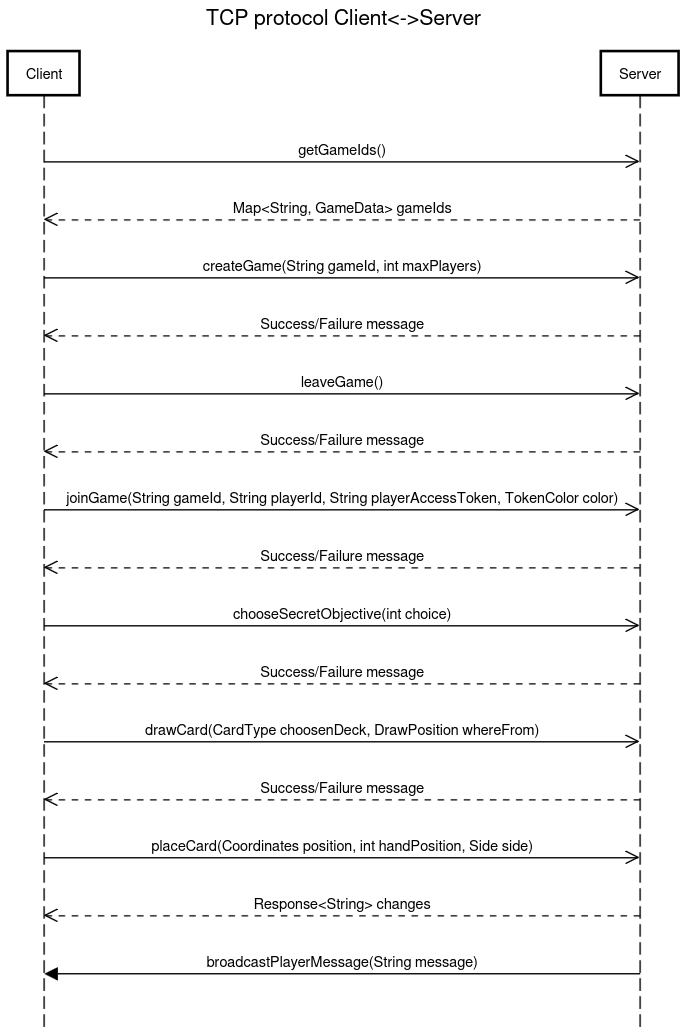
\includegraphics[scale=0.29]{AM30_TCPprotocol.png}
        \caption{Sequence diagram presentato dal gruppo AM30: TCP}
    \end{center}
\end{figure}
\begin{figure}[H]
    \begin{center}
        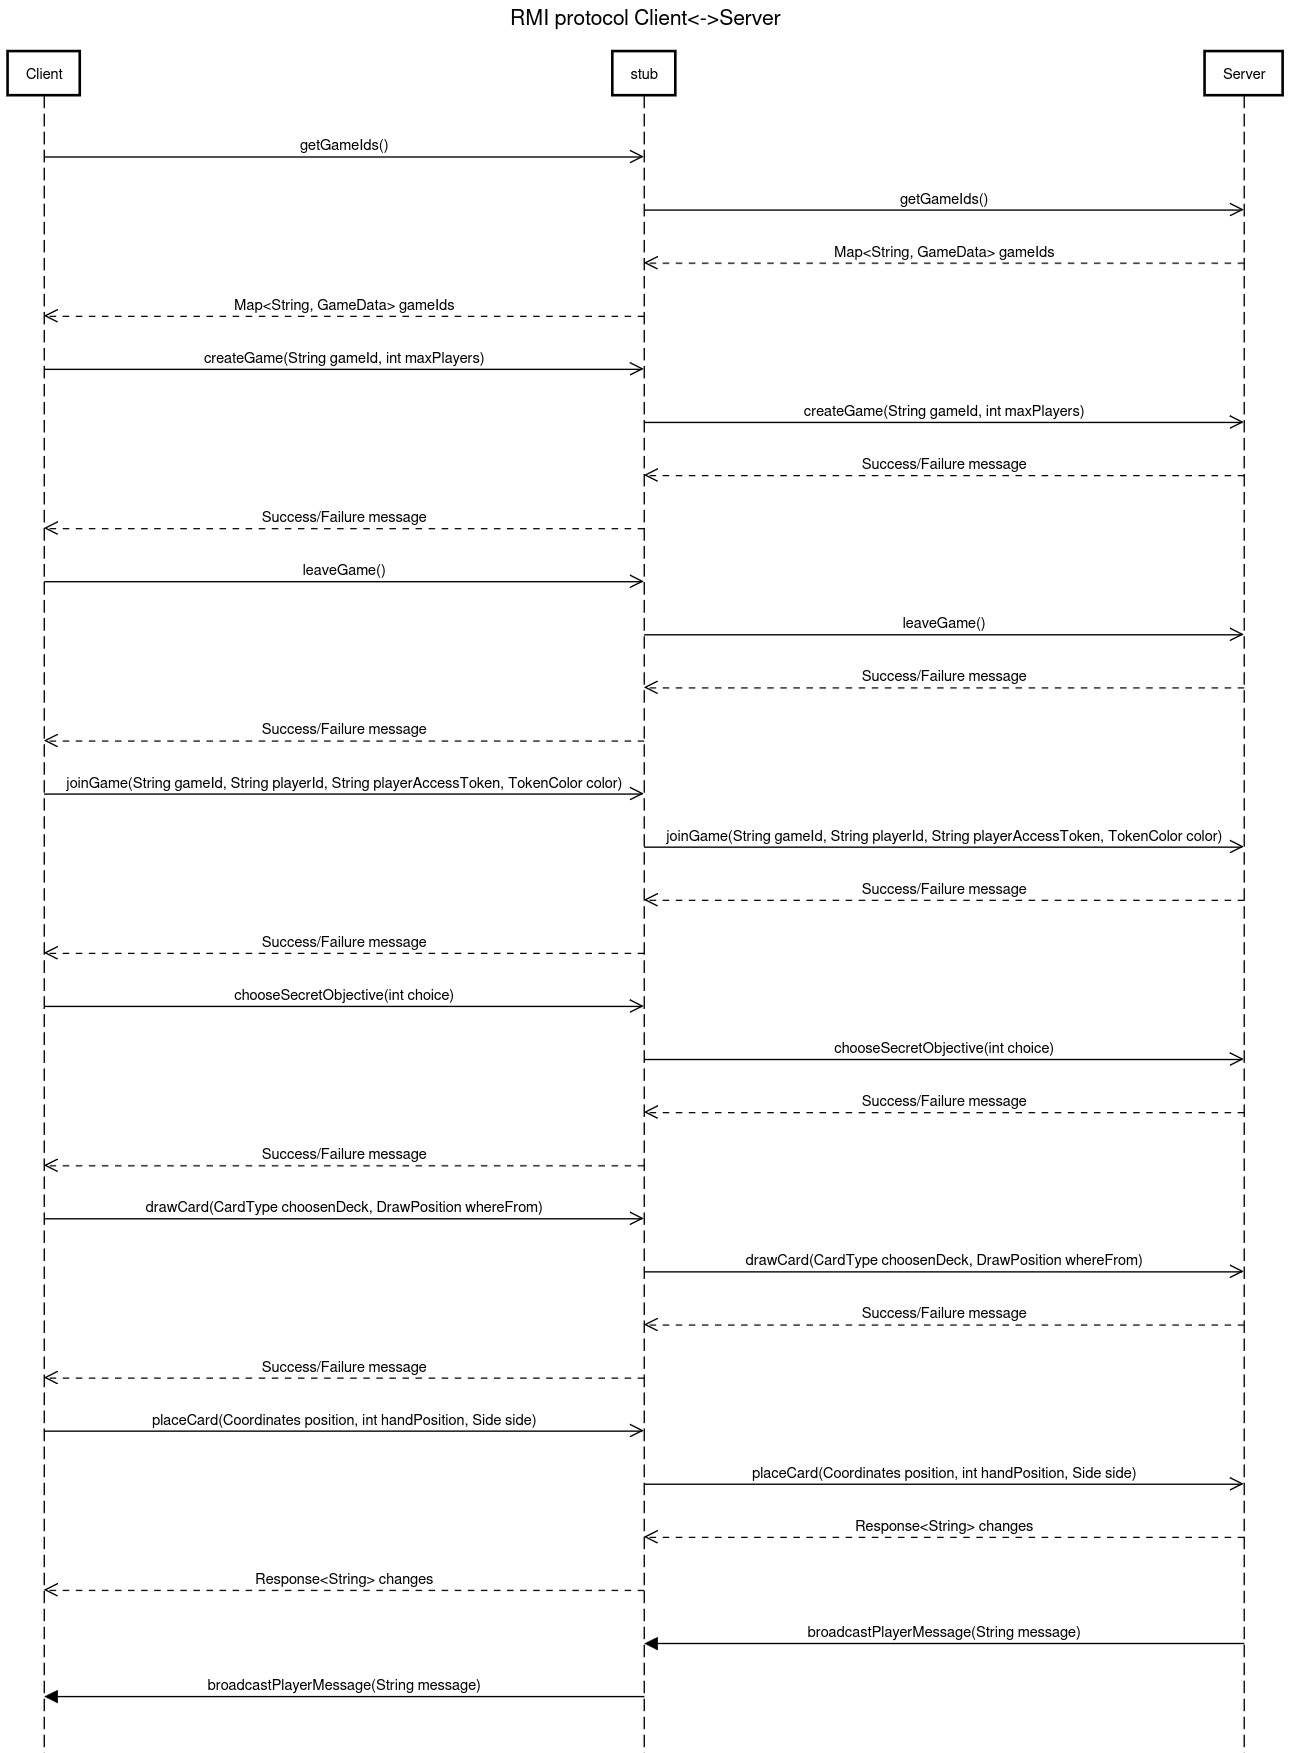
\includegraphics[scale=0.29]{AM30_RMIprotocol.png}
        \caption{Sequence diagram presentato dal gruppo AM30: RMI}
    \end{center}
\end{figure}
\addtocontents{toc}{\setcounter{tocdepth}{3}}
\end{document}
